% para impress�o considerar a troca de oneside para twoside
\documentclass[a4paper, 12pt, openany, oneside, english, brazil]{abntex2}
\usepackage[brazil]{babel}
%\usepackage[utf8]{inputenc}
\usepackage[latin1]{inputenc}
\usepackage[T1]{fontenc}
\usepackage{dsfont}
\usepackage{cmap}
\usepackage{lmodern}
\usepackage{amssymb,amsmath}
\usepackage{multirow}
\usepackage{color, graphicx}
\usepackage{colortbl}
\usepackage{url}
\usepackage{microtype} 			% para melhorias de justifica��o
% Sistema autor-data
\usepackage[alf]{abntex2cite}
% Pacote para o uso de algoritmos
\usepackage[portuguese, ruled, linesnumbered, noline]{algorithm2e}
\newcommand{\curso}[1]{\def\imprimircurso{#1}}
\newcommand{\dataDaAprovacao}[1]{\def\imprimirdatadaaprovacao{#1}}
\newcommand{\tituloEstrangeiro}[1]{\def\imprimirtituloestrangeiro{#1}}

\renewcommand{\imprimircapa}{%
  \begin{capa}
    \begin{center}

      % Cabe�alho (n�o deve ser modificado)
      % Cont�m o bras�o da Universidade, o logotipo do Departamento, al�m dos dados
      % relacionados � vincula��o do aluno (Universidade, Centro, Departamento e Curso)
      \begin{minipage}{2cm}
        \begin{center}
          
\includegraphics[width=1.7cm, height=2.0cm]{imagens/Brasao-UFRN.jpg}
        \end{center}
      \end{minipage}
      \begin{minipage}{11cm}
        \begin{center}
          \begin{SingleSpace}
            {\small \textsc{Universidade Federal do Rio Grande do Norte}
\\
                    \textsc{Centro de Ci�ncias Exatas e da Terra}
\\
                    \textsc{Departamento de Inform�tica e Matem�tica Aplicada}
\\
                    \textsc{Bacharelado em Ci�ncia da Computa��o}}
          \end{SingleSpace}
        \end{center}
      \end{minipage}
      \begin{minipage}{2cm}
        \begin{center}
          
\includegraphics[width=1.8cm, height=1.5cm]{imagens/Logotipo-DIMAp.jpg}
        \end{center}
      \end{minipage}

      \vspace{6cm}

      % T�tulo do trabalho
      {\setlength{\baselineskip}
      {1.3\baselineskip}
      {\LARGE \textbf{\imprimirtitulo}}\par}

      \vspace{4cm}

      % Nome do aluno (autor)

      {\large \textbf{\imprimirautor}}

      \vspace{7cm}

      % Local da institui��o onde o trabalho deve ser apresentado e ano de entrega do mesmo
      \imprimirlocal\\\imprimirdata 
    \end{center}
  \end{capa}

  % Solu��o para gera��o de p�ginas duplicadas, uma delas fica em branco
  \hypersetup{pageanchor=true}
}

% Conteudo padrao da Folha de Rosto
\makeatletter
\renewcommand{\folhaderostocontent} {
  \begin{center}

    {\ABNTEXchapterfont\bfseries\large\imprimirautor}

    \vspace*{\fill}\vspace*{\fill}
    \begin{center}
      \ABNTEXchapterfont\bfseries\Large\imprimirtitulo
    \end{center}
    \vspace*{\fill}

    \abntex@ifnotempty{\imprimirpreambulo}{%
      \hspace{.45\textwidth}
      \begin{minipage}{.5\textwidth}
        \SingleSpacing
          \imprimirpreambulo
      \end{minipage}%
      \vspace*{\fill}
    }%

    {\large\imprimirorientadorRotulo~\par\imprimirorientador\par}
    \abntex@ifnotempty{\imprimircoorientador}{%
      {\large\imprimircoorientadorRotulo~\imprimircoorientador}
    }%
    \vspace*{\fill}

    {\abntex@ifnotempty{\imprimirinstituicao}{%
      \textsc{\imprimirinstituicao}\vspace*{\fill}}%
    }

    {\large\imprimirlocal}
    \par
    {\large\imprimirdata}
    \vspace*{1cm}

  \end{center}
}
\makeatother

%% Redefinicao de instrucoes
\floatname{algorithm}{Algoritmo}
\renewcommand{\algorithmicrequire}{\textbf{Entrada:}}
\renewcommand{\algorithmicensure}{\textbf{Saída:}}
\renewcommand{\algorithmicend}{\textbf{fim}}
\renewcommand{\algorithmicif}{\textbf{se}}
\renewcommand{\algorithmicthen}{\textbf{então}}
\renewcommand{\algorithmicelse}{\textbf{senão}}
\renewcommand{\algorithmicfor}{\textbf{para}}
\renewcommand{\algorithmicforall}{\textbf{para todo}}
\renewcommand{\algorithmicdo}{\textbf{faça}}
\renewcommand{\algorithmicwhile}{\textbf{enquanto}}
\renewcommand{\algorithmicloop}{\textbf{loop}}
\renewcommand{\algorithmicrepeat}{\textbf{repetir}}
\renewcommand{\algorithmicuntil}{\textbf{até que}}
\renewcommand{\algorithmiccomment}[1]{\% #1}

% \listofalgorithms: comando que imprime a lista de algoritmos
\renewcommand{\listalgorithmname}{Lista de algoritmos}

% Redefinindo as cores dos links (pacote hyperref)
% O hyperref é incluso automaticamente pelo abntex2
\hypersetup{pageanchor=false,
              colorlinks=true,
              linkcolor=black,
              citecolor=black,
              urlcolor=blue}


% Redefinicao de alguns comandos do pacote algorithm2e
\SetKwBlock{Inicio}{in\'{i}cio}{fim}
\SetKwFor{Para}{para}{fa\c{c}a}{fim para}%
\SetKwFor{ParaCada}{para cada}{fa\c{c}a}{fim para}%
\SetKwIF{Se}{SenaoSe}{Senao}{se}{ent\~{a}o}{sen\~{a}o se}{sen\~{a}o}{fim se}%
\SetKwRepeat{Repita}{repita}{at\'{e}}%

% espaçamento entre linhas 1.5cm segundo ABNT, por padrão a classe antex2 já é 1.5.
% \OnehalfSpacing (padrão) or \DoubleSpace para mudar
% Recuo do parágrafo em 1.5cm
\setlength{\parindent}{1.5cm}

% Texto padrão fontes do capítulo em Latin Mordern Roman (lmodern), mesma fonte usada no texto
\renewcommand{\ABNTEXchapterfont}{\fontfamily{lmr}\fontseries{b}\selectfont}

% Dados pessoais
\autor{Nome do aluno}
\curso{Ciência da Computação}

% Dados do trabalho
\titulo{Título do trabalho}
\tituloEstrangeiro{Título do trabalho (em língua estrangeira)}
\data{Mês (por extenso) e ano}
%\palavraChaveUm{Palavra-chave01}
%\palavraChaveDois{Palavra-chave02}

% Dados da orientacao
\orientador[Orientador(a)]{Titulação e nome do(a) orientador(a)}
%\coorientador{(quando houver, Titulação Acadêmica e Nome do Orientador)}

% Dados da aprovação do trabalho
\dataDaAprovacao{data de aprovação (por extenso)} % 01 de junho de 2016
%\membroConvidadoUm{Titulação e Nome do Professor Convidado 01}
%\membroConvidadoDois{Titulação e Nome do Professor Convidado 02}

\local{Natal-RN}
\instituicao{%
  Universidade Federal do Rio Grande do Norte -- UFRN
  \par
  Departamento de Inform�tica e Matem�tica Aplicada -- DIMAp
}
\tipotrabalho{Trabalho de Conclus�o de Curso}
\preambulo{Monografia de Gradua��o apresentada ao Departamento de Inform�tica e Matem�tica Aplicada do Centro de Ci�ncias Exatas e da Terra da Universidade Federal do Rio Grande do Norte como requisito parcial para a obten��o do grau de bacharel em \imprimircurso.}


% Hifenização de palavras feita de forma incorreta pelo LaTeX
\hyphenation{PYTHON ou-tros}

% Inicio do documento

\begin{document}

  \frenchspacing
  \imprimircapa
  \imprimirfolhaderosto

  % Folha de aprovação
\begin{folhadeaprovacao}
  \setlength{\ABNTEXsignthickness}{0.4pt}
  \setlength{\ABNTEXsignwidth}{10cm}
  \setlength{\ABNTEXsignskip}{2.5cm}

  % Informações gerais acerca do trabalho
  % (nome do autor, título, instituição à qual é submetido e natureza)
  \noindent
  Monografia de Graduação sob o título \textit{\imprimirtitulo} apresentada por \imprimirautor e aceita pelo Departamento de Informática e Matemática Aplicada do Centro de Ciências Exatas e da Terra da Universidade Federal do Rio Grande do Norte, sendo aprovada por todos os membros da banca examinadora abaixo especificada:

  % Membros da banca examinadora e respectivas filiações
  \assinatura
  {
    \imprimirorientador\\
    {\small Orientador(a)}\\
    {\footnotesize
      Departamento\\
      Universidade
    }
  }

  \assinatura
  {
    Titulação e nome do membro da banca examinadora\\
    {\small Co-orientador(a), se houver}\\
    {\footnotesize
      Departamento\\
      Universidade
    }
  }

  \assinatura
  {
    Titulação e nome do membro da banca examinadora\\
    {\footnotesize
      Departamento\\
      Universidade
    }
  }

  \assinatura
  {
    Titulação e nome do membro da banca examinadora\\
    {\footnotesize
      Departamento\\
      Universidade
    }
  }

  \vfill

  \begin{center}
    \imprimirlocal, \imprimirdatadaaprovacao.
  \end{center}
\end{folhadeaprovacao}

  \begin{dedicatoria}
  \vspace*{\fill}
  \centering
  \noindent
     Homenagem que o autor presta a uma ou mais pessoas.
  \vspace*{\fill}
\end{dedicatoria}
  % Agradecimentos

\begin{agradecimentos}
  Agradecimentos dirigidos àqueles que contribuíram de maneira relevante à elaboração do trabalho, sejam eles pessoas ou mesmo organizações.
\end{agradecimentos}
  % Ep�grafe (cita��o seguida de indica��o de autoria)
\begin{epigrafe}
  \vspace*{\fill}
  \begin{flushright}
    \textit
    {
      Cita��o
    }\medskip\\
    Autor
  \end{flushright}
\end{epigrafe}
  % Resumo em l�ngua vern�cula
\begin{center}
  {\Large{\textbf{\imprimirtitulo}}}
\end{center}

\vspace{1cm}

\begin{flushright}
  Autor: \imprimirautor\\
  \imprimirorientadorRotulo~: \imprimirorientador
\end{flushright}

\vspace{1cm}

\begin{resumo}[RESUMO]
  O resumo deve apresentar de forma concisa os pontos relevantes de um texto, fornecendo uma vis�o r�pida e clara do conte�do e das conclus�es do trabalho. O texto, redigido na forma impessoal do verbo, � constitu�do de uma seq��ncia de frases concisas e objetivas e n�o de uma simples enumera��o de t�picos, n�o ultrapassando 500 palavras, seguido, logo abaixo, das palavras representativas do conte�do do trabalho, isto �, palavras-chave e/ou descritores. Por fim, deve-se evitar, na reda��o do resumo, o uso de par�grafos (em geral resumos s�o escritos em par�grafo �nico), bem como de f�rmulas, equa��es, diagramas e s�mbolos, optando-se, quando necess�rio, pela transcri��o na forma extensa, al�m de n�o incluir cita��es bibliogr�ficas.
  \vspace{\onelineskip}

  \noindent
  \textit{Palavras-chave}: Palavra-chave 1, Palavra-chave 2, Palavra-chave 3.
\end{resumo}
  % Resumo em língua estrangeira (em inglês Abstract, em espanhol Resumen, em francês Résumé)
\begin{center}
  {\Large{\textbf{\imprimirtituloestrangeiro}}}
\end{center}

\vspace{1cm}

\begin{flushright}
  Author: \imprimirautor\\
  Advisor: \imprimirorientador
\end{flushright}

\vspace{1cm}

\begin{resumo}[ABSTRACT]
  \begin{otherlanguage*}{english}
    O resumo em língua estrangeira (em inglês \textit{Abstract}, em espanhol \textit{Resumen}, em francês \textit{Résumé}) é uma versão do resumo escrito na língua vernácula para idioma de divulgação internacional. Ele deve apresentar as mesmas características do anterior (incluindo as mesmas palavras, isto é, seu conteúdo não deve diferir do resumo anterior), bem como ser seguido das palavras representativas do conteúdo do trabalho, isto é, palavras-chave e/ou descritores, na língua estrangeira. Embora a especificação abaixo considere o inglês como língua estrangeira (o mais comum), não fica impedido a adoção de outras linguas (a exemplo de espanhol ou francês) para redação do resumo em língua estrangeira.

    \vspace{\onelineskip}

    \noindent
    \textit{Keywords}: Keyword 1, Keyword 2, Keyword 3.
  \end{otherlanguage*}
\end{resumo}



  % Lista de ilustrações e tabelas
  \pdfbookmark[0]{\listfigurename}{lof}
\listoffigures*
\cleardoublepage
\pdfbookmark[0]{\listtablename}{lot}
\listoftables*
\cleardoublepage

% ------------------------
%   LISTA DE ABREVIATURAS
% ------------------------

\newcommand{\abrv}[2][]{%
  \ifthenelse{\equal{#1}{}}
  {\addcontentsline{loab}{abreviatura}{#2}}
  {\addcontentsline{loab}{abreviatura}{#1}}#2}
% Para aceitar comandos com @ (at) no nome
\makeatletter
% \listadeabreviaturas: comando que imprime a lista de abreviaturas e siglas
\newcommand{\listadeabreviaturas}
{
  \pretextualchapter{Lista de abreviaturas e siglas}
  {\setlength{\parindent}{0cm}
  \@starttoc{loab}}
}
% Como a entrada sera impressa
\newcommand\l@abreviatura[2]{\par #1}
\makeatother


  % Lista de abreviaturas e siglas
  \begin{siglas}
  \item[UFRN] Universidade Federal do Rio Grande do Norte
  \item[DIMAp] Departamento de Inform�tica e Matem�tica Aplicada
\end{siglas}


  % Lista de símbolos
  \begin{simbolos}
  \item[$ \lambda $] (algum simbolo)
\end{simbolos}

  % Lista de algoritmos (se houver)
  % Devem ser incluídos os pacotes algorithm e algorithmic
  \listofalgorithms
  \newpage
	
  % Sumário
  \pdfbookmark[0]{\contentsname}{toc}
\tableofcontents*
\cleardoublepage

  % Parte central do trabalho, englobando os capítulos que constituem o mesmo
  % Os referidos capítulos devem ser organizados dentro do diretório "Capítulos"
  \textual

  % Capitulo 1: Introdução (arquivo capitulos/introducao.tex)
  % Introdu��o
\chapter{Introdu��o}

A introdu��o � a parte inicial do texto e que possibilita uma vis�o geral de todo o trabalho, devendo constar a delimita��o do assunto tratado, objetivos da pesquisa, motiva��o para o desenvolvimento da mesma e outros elementos necess�rios para situar o tema do trabalho.

\section{Organiza��o do trabalho}

Nesta se��o deve ser apresentado como est� organizado o trabalho, sendo descrito, portanto, do que trata cada cap�tulo.

  % Capitulo 2: Segundo capítulo (arquivo capitulos/capitulo2.tex)
  % Cap�tulo 2
\chapter{Cap�tulo 2}

Este � o primeiro cap�tulo da parte central do trabalho, isto �, o desenvolvimento, a parte mais extensa de todo o trabalho. Geralmente o desenvolvimento � dividido em cap�tulos, cada um com subse��es e subse��es, cujo tamanho e n�mero de divis�es variam em fun��o da natureza do conte�do do trabalho.

Em geral, a parte de desenvolvimento � subdividida em quatro subpartes:
\begin{itemize}
	\item \textit{contextualiza��o ou defini��o do problema} -- consiste em descrever a situa��o ou o contexto geral referente ao assunto em quest�o, devem constar informa��es atualizadas visando a proporcionar maior consist�ncia ao trabalho;
	\item \textit{referencial ou embasamento te�rico} -- texto no qual se deve apresentar os aspectos te�ricos, isto �, os conceitos utilizados e a defini��o dos mesmos; nesta parte faz-se a revis�o de literatura sobre o assunto, resumindo-se os resultados de estudos feitos por outros autores, cujas obras citadas e consultadas devem constar nas refer�ncias;
	\item \textit{metodologia do trabalho ou procedimentos metodol�gicos} -- deve constar o instrumental, os m�todos e as t�cnicas aplicados para a elabora��o do trabalho;
	\item \textit{resultados} -- devem ser apresentados, de forma objetiva, precisa e clara, tanto os resultados positivos quanto os negativos que foram obtidos com o desenvolvimento do trabalho, sendo feita uma discuss�o que consiste na avalia��o circunstanciada, na qual se estabelecem rela��es, dedu��es e generaliza��es.
\end{itemize}

� recomend�vel que o n�mero total de p�ginas referente � parte de desenvolvimento n�o ultrapasse 60 (sessenta) p�ginas.

\section{Se��o 1}

Teste de figura:

\begin{figure}[htb]
	\centering
  	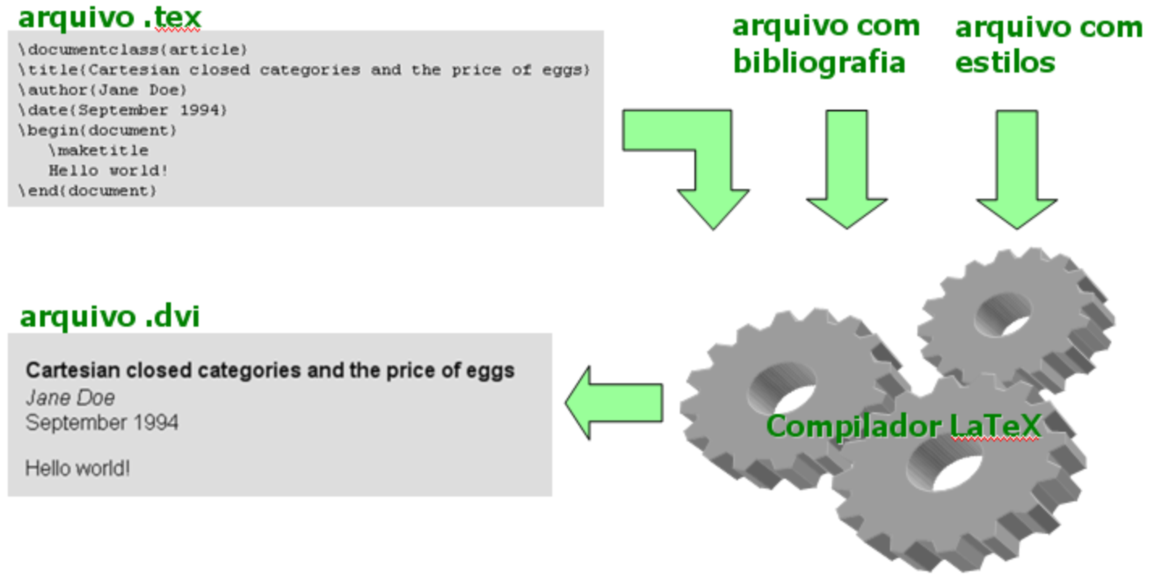
\includegraphics[scale=7.0]{imagens/FiguraTeste.png}
  	\textsf{\caption{Teste de uma figura em formato .png}}
  	\label{fig:FiguraTeste}
\end{figure}


\section{Se��o 2}

Referenciamento da figura inserida na se��o anterior: \ref{fig:FiguraTeste}


\section{Se��o 3}

Se��o 3


\section{Se��o 4}

Se��o 4


  % Capitulo 3: Terceiro capítulo (arquivo capitulos/capitulo3.tex)
  % Capítulo 3
\chapter{Capítulo 3}

Algumas regras devem ser observadas na redação da monografia:
\begin{enumerate}
	\item ser claro, preciso, direto, objetivo e conciso, utilizando frases curtas e evitando ordens inversas desnecessárias;
	\item construir períodos com no máximo duas ou três linhas, bem como parágrafos com cinco linhas cheias, em média, e no máximo oito (ou seja, não construir parágrafos e períodos muito longos, pois isso cansa o(s) leitor(es) e pode fazer com que ele(s) percam a linha de raciocínio desenvolvida);
	\item a simplicidade deve ser condição essencial do texto; a simplicidade do texto não implica necessariamente repetição de formas e frases desgastadas, uso exagerado de voz passiva (como \textit{será iniciado}, \textit{será realizado}), pobreza vocabular etc. Com palavras conhecidas de todos, é possível escrever de maneira original e criativa e produzir frases elegantes, variadas, fluentes e bem alinhavadas;
	\item adotar como norma a ordem direta, por ser aquela que conduz mais facilmente o leitor à essência do texto, dispensando detalhes irrelevantes e indo diretamente ao que interessa, sem rodeios (verborragias);
	\item não começar períodos ou parágrafos seguidos com a mesma palavra, nem usar repetidamente a mesma estrutura de frase;
	\item desprezar as longas descrições e relatar o fato no menor número possível de palavras;
	\item recorrer aos termos técnicos somente quando absolutamente indispensáveis e nesse caso colocar o seu significado entre parênteses (ou seja, não se deve admitir que todos os que lerão o trabalho já dispõem de algum conhecimento desenvolvido no mesmo);
	\item dispensar palavras e formas empoladas ou rebuscadas, que tentem transmitir ao leitor mera idéia de erudição;
	\item não perder de vista o universo vocabular do leitor, adotando a seguinte regra prática: \textit{nunca escrever o que não se diria};
	\item termos coloquiais ou de gíria devem ser usados com \textit{extrema} parcimônia (ou mesmo nem serem utilizados) e apenas em casos muito especiais, para não darem ao leitor a idéia de vulgaridade e descaracterizar o trabalho;
	\item ser rigoroso na escolha das palavras do texto, desconfiando dos sinônimos perfeitos ou de termos que sirvam para todas as ocasiões; em geral, há uma palavra para definir uma situação;
	\item encadear o assunto de maneira suave e harmoniosa, evitando a criação de um texto onde os parágrafos se sucedem uns aos outros como compartimentos estanques, sem nenhuma fluência entre si;
	\item ter um extremo cuidado durante a redação do texto, principalmente com relação às regras gramaticais e ortográficas da língua; geralmente todo o texto é escrito na forma impessoal do verbo, não se utilizando, portanto, de termos em primeira pessoa, seja do plural ou do singular.
\end{enumerate}


\section{Seção 1}

Teste de uma tabela:

\begin{table}[htb]
	% Título de tabelas sempre aparecem antes da tabela
	\textsf{\caption{Tabela sem sentido}}
	\center
	{
		\begin{tabular}{l|l}
			\hline
			Titulo Coluna 1   & Título Coluna 2\\
			\hline
			X                 & Y\\
			X                 & W\\
			\hline
		\end{tabular}
	}
	\label{tab:TabelaSemSentido}
\end{table}


\section{Seção 2}

Seção 2


\subsection{Subseção 2.1}

Referência à tabela definida no início: \ref{tab:TabelaSemSentido}


\subsection{Subseção 2.2}

Subsection 2.2


\section{Seção 3}

Seção 3

  % Capitulo 4: Quarto capítulo (arquivo capitulos/capitulo4.tex)
  % Capítulo 4
\chapter{Capítulo 4}

\section{Seção 1}

Teste para símbolo

$\lambda$
%\simb[$\lambda$ (algum símbolo)]{$\lambda$}


\section{Seção 2}

Teste para abreviatura 

\abrv[UFRN -- Universidade Federal do Rio Grande do Norte]{UFRN}

\abrv[DIMAp -- Departamento de Informática e Matemática Aplicada]{DIMAp}


  % Capitulo 5: Quinto capítulo (arquivo capitulos/capitulo5.tex)
  % Capítulo 5
\chapter{Capítulo 5}

\section{Exemplo de algoritmo}

O Algoritmo \ref{alg:howto} usa o pacote {\texttt algorithm2e} que suporta comandos em Português.

\begin{algorithm}[H]
    \SetAlgoLined
    \Entrada{Entrada do algoritmo}
    \Saida{Saída do Algoritmo}
    \Inicio{
        inicialização\;
        \Enqto{condição}{
        instrução\;
        \eSe{condição}{
            instrução1\;
            instrução2\;
        }{
            instrução3\;
        }
        }
        \Para{i de 1 até 10}{
        instrução\;
        }
    }
    \caption{Como escrever algoritmos}
    \label{alg:howto}
\end{algorithm}


\section{Seção 2}

Alguns exemplos de citação: 

Na tese de Doutorado de Paquete \cite{PaquetePhD}, discute-se sobre algoritmos de busca local estocásticos aplicados a problemas de Otimização Combinatória considerando múltiplos objetivos. Por sua vez, o trabalho de \cite{KnowlesBoundedLebesgue}, publicado nos anais do IEEE CEC de 2003, mostra uma técnica de arquivamento também empregada no desenvolvimento de algoritmos evolucionários multi-objetivo, trabalho esse posteriormente estendido para um capítulo de livro dos mesmos autores \cite{KnowlesBoundedPareto}. Por fim, no relatório técnico de \citeonline{Jaszkiewicz}, fala-se sobre um algoritmo genético híbrido para problemas multi-critério, enquanto no artigo de jornal de Lopez \textit{et al.} \cite{LopezPaqueteStu} trata-se do \textit{trade-off} entre algoritmos genéticos e metodologias de busca local, também aplicados no contexto multi-critério e relacionado de alguma forma ao trabalho de Jaszkiewicz (\citeyear{Jaszkiewicz}).

Outros exemplos relacionados encontram-se em \cite{Silberschatz} (livro), \cite{DB2XML} (referência da Web) e \cite{Angelo} (dissertação de Mestrado).

\subsection{Subseção 5.1}

Subseção 5.1

\subsection{Subseção 5.2}

Subsection 5.2

\section{Seção 3}

Seção 3

  % Consideracoes finais
  % Considera��es finais
\chapter{Considera��es finais}

As considera��es finais formam a parte final (fechamento) do texto, sendo dito de forma resumida (1) o que foi desenvolvido no presente trabalho e quais os resultados do mesmo, (2) o que se p�de concluir ap�s o desenvolvimento bem como as principais contribui��es do trabalho, e (3) perspectivas para o desenvolvimento de trabalhos futuros. O texto referente �s considera��es finais do autor deve salientar a extens�o e os resultados da contribui��o do trabalho e os argumentos utilizados estar baseados em dados comprovados e fundamentados nos resultados e na discuss�o do texto, contendo dedu��es l�gicas correspondentes
aos objetivos do trabalho, propostos inicialmente.

  \postextual
  
  % Bibliografia (arquivo capitulos/referencias.bib)
  \bibliography{capitulos/referencias}
  % Sistema autor-data
  \bibliographystyle{abntex2-alf}
  % Sistema numérico
  %\bibliographystyle{abntex2-num}

  % Apêndice A (arquivo capitulos/apendices.tex)
  % Ap�ndice
\begin{apendicesenv}

  \partapendices

  \chapter{Primeiro ap�ndice}

  Os ap�ndices s�o textos ou documentos elaborados pelo autor, a fim de complementar sua argumenta��o, sem preju�zo da unidade nuclear do trabalho.

\end{apendicesenv}


  % Anexo A (arquivo capitulos/anexos.tex)
  % Anexo
\begin{anexosenv}

  \partanexos

  \chapter{Primeiro anexo}

  Os anexos s�o textos ou documentos n�o elaborado pelo autor, que servem de fundamenta��o, comprova��o e ilustra��o.
\end{anexosenv}


  % Página em branco
  \newpage
\end{document}
